\chapter{Specyfikacja zewnętrzna}
\label{ch:04}

\paragraph{}
Aplikacja do działania potrzebuje serwera - komputera, na którym skompilowany z kodu źródłowego program, jak również baza danych, będą uruchomione. Serwer musi posiadać dostęp do internetu oraz jego adres musi być publicznie dostępny. Dzięki temu ma on możliwość obsługiwania żądań HTTP wysyłanych przez uzytkowników.

\paragraph{}
W przypadku działającego serwera, można do użytkowania aplikacji. W celu uzyskania do niej dostępu, użytkownik musi mieć zainstalowaną przeglądarkę na urządzeniu (np. komputerze stacjonarnym, laptopie, tablecie czy smartfonie) oraz połączenia z internetem. Po spełnieniu powyższych wymagań, w pasek adresu URL w przeglądarce należy wpisać adres serwera oraz port, na którym uruchomiona jest aplikacja. Można również uprościć użytkownikom uruchomienie aplikacji poprzez uruchomienie serwera na konkretnej domenie DNS, którą wystarczy wpisać w przeglądarce, natomiast nie zostało to zaimplementowane w trakcie procesu tworzenia systemu.

\paragraph{}
Wyróżniamy dwa rodzaje użytkowników: 
\begin{itemize}
	\item niezalogowany użytkownik
	\item zalogowany użytkownik
\end{itemize}

\paragraph{}
Z niezalogowanym użytkownikiem mamy do czynienia wówczas, gdy nastąpi włączenie aplikacji lub po wylogowaniu się ze swojego konta podczas użytkowania. Funkcje, które ma on do dyspozycji, są mocno ograniczone. Użytkownik ma wtedy dostęp do:
\begin{itemize}
	\item strony głównej - tylko wyświetla tekst 
	\item formularza rejestracji - pozwala utworzyć konto użytkownika
	\item formularza logowania - umożliwia zalogowanie się na istniejące w systemie konto
\end{itemize}

\paragraph{}
Zalogowany użytkownik uzyskuje dostęp do właściwych funkcji systemu, dzięki którym może zarządzać lokalizatorami, jak również kierowcami i pojazdami.

\paragraph{}
Po włączeniu aplikacji ukazuje się strona główna. Widczony na niej tekst zachęca do skorzystania z wszystkich funkcji systemu. Jej wygląd jest widoczny na rys. 4.1. Na górze strony znajduje się pasek nawigacji, który towarzyszy użytkownikowi przez cały czas użytkowania programu, lecz różni się w zależności od tego, czy użytkownik jest niezalogowany (pasek wtedy przybiera formę jak na rys. 4.1), czy zalogowany (w tym przypadku pasek wygląda jak na rys. 4.4). Po kliknięciu w poszczególną opcję na pasku, odpowiadająca jej zakładka jest otwierana. Aby przejść do formularzy logowania i rejestracji, należy wybrać opcję ""


Jeśli „Specyfikacja zewnętrzna”:
\begin{itemize}
\item  wymagania sprzętowe i programowe
\item  sposób instalacji
\item  sposób aktywacji
\item  kategorie użytkowników
\item  sposób obsługi
\item  administracja systemem
\item  kwestie bezpieczeństwa
\item  przykład działania
\item  scenariusze korzystania z systemu (ilustrowane zrzutami z ekranu lub generowanymi dokumentami)
\end{itemize}

%%%%%%%%%%%%%%%%%%%%%
%% RYSUNEK Z PLIKU
%
%\begin{figure}
%\centering
%\includegraphics[width=0.5\textwidth]{./graf/politechnika_sl_logo_bw_pion_pl.pdf}
%\caption{Podpis rysunku zawsze pod rysunkiem.}
%\label{fig:etykieta-rysunku}
%\end{figure}
%Rys. \ref{fig:etykieta-rysunku} przestawia …
%%%%%%%%%%%%%%%%%%%%%
%
%%%%%%%%%%%%%%%%%%%%%
%% WIELE RYSUNKÓW 
%
%\begin{figure}
%\centering
%\begin{subfigure}{0.4\textwidth}
%    \includegraphics[width=\textwidth]{./graf/politechnika_sl_logo_bw_pion_pl.pdf}
%    \caption{Lewy górny rysunek.}
%    \label{fig:lewy-gorny}
%\end{subfigure}
%\hfill
%\begin{subfigure}{0.4\textwidth}
%    \includegraphics[width=\textwidth]{./graf/politechnika_sl_logo_bw_pion_pl.pdf}
%    \caption{Prawy górny rysunek.}
%    \label{fig:prawy-gorny}
%\end{subfigure}
%
%\begin{subfigure}{0.4\textwidth}
%    \includegraphics[width=\textwidth]{./graf/politechnika_sl_logo_bw_pion_pl.pdf}
%    \caption{Lewy dolny rysunek.}
%    \label{fig:lewy-dolny}
%\end{subfigure}
%\hfill
%\begin{subfigure}{0.4\textwidth}
%    \includegraphics[width=\textwidth]{./graf/politechnika_sl_logo_bw_pion_pl.pdf}
%    \caption{Prawy dolny rysunek.}
%    \label{fig:prawy-dolny}
%\end{subfigure}
%        
%\caption{Wspólny podpis kilku rysunków.}
%\label{fig:wiele-rysunkow}
%\end{figure}
%Rys. \ref{fig:wiele-rysunkow} przestawia wiele ważnych informacji, np. rys. \ref{fig:prawy-gorny} jest na prawo u góry.
%%%%%%%%%%%%%%%%%%%%%


 
\begin{figure}
\centering
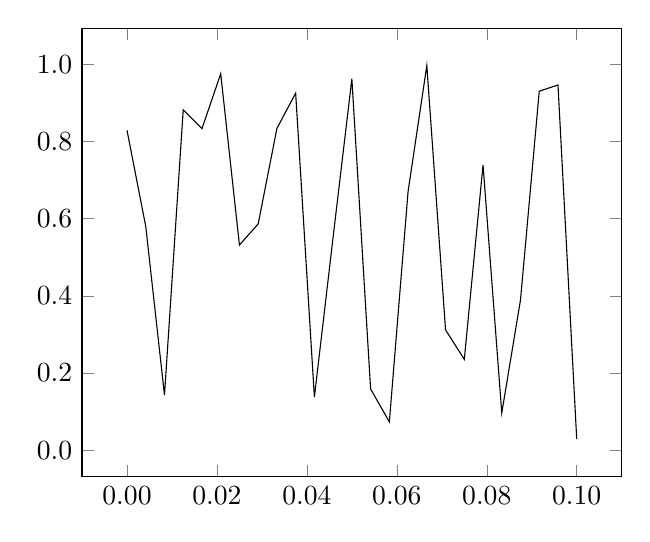
\begin{tikzpicture}
\begin{axis}[
    y tick label style={
        /pgf/number format/.cd,
            fixed,   % po zakomentowaniu os rzednych jest indeksowana wykladniczo
            fixed zerofill, % 1.0 zamiast 1
            precision=1,
        /tikz/.cd
    },
    x tick label style={
        /pgf/number format/.cd,
            fixed,
            fixed zerofill,
            precision=2,
        /tikz/.cd
    }
]
\addplot [domain=0.0:0.1] {rnd};
\end{axis} 
\end{tikzpicture}
\caption{Podpis rysunku po rysunkiem.}
\label{fig:2}
\end{figure}

